\chapter{Researching homogeneous temporal periods}\label{chp:3}

\minitoc

\clearpage

Although the recommendations for the use of the substances are formulated in the marketing authorization issued by ANSES \cite{ephy}, their practical use is not subject to the control of the agency. Cultivation practises depend on meteorological conditions and professional habits. This partly explains the spatiotemporal heterogeneity. Our goal is to find homogeneous time periods and geographic areas and make a statistical comparison of these regions in these stable time periods to support the expert analysis. In this chapter, we focus on identifying stable temporal patterns using change point detection methods. This mathematical area is covered by several surveys \cite{truong2020,basseville1993detection}. We have focused on those methods that seem appropriate for the application area of phytopharmacovigilance. For example, this work will focus only on the offline methods that we will develop in the following sections. This choice was motivated by the speed of data collection and storage of pesticides concentrations data. Nevertheless, for readers who wish to refer to it, we can state that there is no shortage of online detection methods in the literature \cite{liu2017change,Li2021,hohle2010online,ranganathan2010pliss,li2015m}.

\section{Model and cost functions}\label{chp:3:1}

We describe the most general configuration of a change-point model suitable for concentration data. We consider a signal consisting of observations $\bm y = (y_1,...,y_n)$, which are the realisations of random variables $Y_1,...,Y_n$. The variables $Y_i$ are recorded sequentially, and the recording times are not necessarily equidistant. Thus, the indices in $Y_i$ are only indicators of the order of occurrence in the sample and not of the observation times. Some properties (trend, mean, variance, etc...) of the signal $\bm y$ are supposed to change at the time points $t_1 <... < t_k <... < t_{K}$. We use the following convention, let $t_0 = 1$ and $t_{K+1} = n$. The purpose of breakpoint detection is to estimate the positions $t_k$ and the number of breaks $K$ when they are unknown. The goal is to identify the data segments in which these properties are stable. We denote $y_{u:v}$ as a segment of the signal from the u-th coordinate to the v-th.  \\
According to the nomenclature proposed by \cite{truong2020}, the change point detection methods operate using a cost function $W$. This function associates a cost to the segment it is evaluated on. intuitively, the more properties (on which changes are investigated) of the segment $y_{u:v}$ are homogenous, the lower the cost $W(y_{u:v})$ is. We define $\mathcal{T}_{K} = \{\bm t = \{t_0 = 1,t_1,\dots,t_k,\dots,t_K,t_{K+1} = n\} \lvert t_0 <\dots < t_k < \dots < t_{K+1} \}$ the set of all possible segmentations of $\bm y$ into $K+1$ segments. The total cost $\mathcal{C}(\bm y,\bm t)$ associated to a segmentation $\bm t \in \TT_K$ is defined as the sum of the costs of all segments:  

\begin{equation}\label{chp:3:costfunc}
\mathcal{C}(\bm y,\bm t) = \sum_{k=0}^K W(y_{t_k:t_{k+1}}), 
\end{equation}     

With these notations and the knowledge of the number of change points $K$ that occurred in $\bm y$, the change point problem can be posed as an optimization problem:

\begin{equation}\label{chp:3:optKknown}
 \widehat{\bm t}  = \arg \min_{\bm t \in\TT_K}  \CC(\bm y, \bm t) = \arg \min_{\bm t \in \TT_K} \sum_{k=0}^K W(y_{t_k:t_{k+1}})   
\end{equation}

The choice of cost function determines the type of changes (in trend, mean, etc.) targeted by the detection. Figure \ref{fig:ex_cp} illustrates two different types of changes that may be of interest for change point detection. In the next parts of this section, we distinguish the cost functions according to the statistical inferences on which they are based. We give a non-exhaustive list of cost functions for each inference.

\begin{figure}[ht]
    \centering
    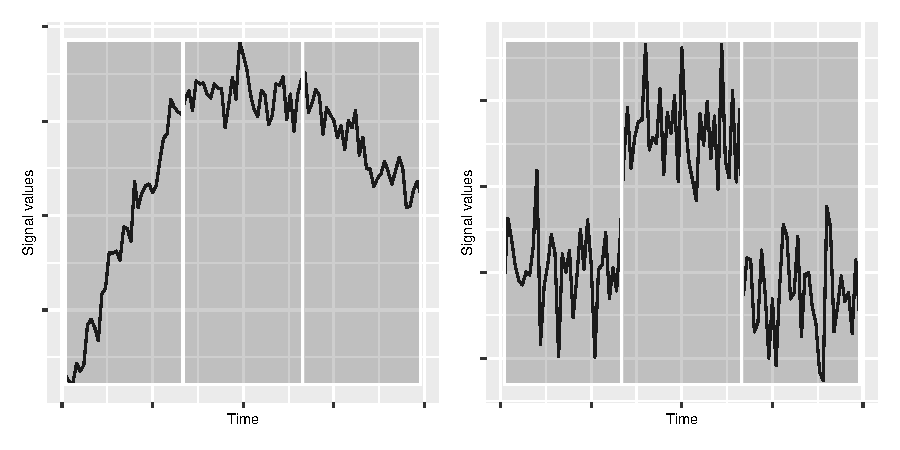
\includegraphics{figs/Chap2/Ex_CP_cost.pdf}
    \caption{Examples of types of change point detection. The figure on the left illustrates changes in trend whereas the figure on the right illustrates changes in mean.}
    \label{fig:ex_cp}
\end{figure}

\subsection{Parametric inference}

In the parametric case, the detection depends heavily on what we are looking for in the signal $\bm y$. For example, searching for slope changes in a signal \cite{Bai1994,Fearnhead2018} does not require the same modelling as detecting changes in the mean \cite{Frick2014,chen2012parametric}. 

A first classical cost function is based on the maximum likelihood estimation. In this setting, the observations located in the $k$-th segment is supposed to be following a distribution $Q$ depending on a set of parameters $\bm \theta_k$. More formally, we have that:
$$y_t \sim f(.;\bm \theta_k)\mathbbm{1}_{t_{k}+1\leq t \leq t_{k+1}},$$
with $f$ being the density function of distribution $Q$. In other words, we suppose that all observations emanate from the same distribution $Q$ but the values of $\bm \theta_k$ change abruptly at each change-point $t_k$. The cost function used to evaluate segments in this context is the negative log-likelihood. Hence, for a segment $y_{u:v}$ with $u < v$, we can write:  
$$W(y_{u:v}) = -\sup_{\bm \theta \in \Theta} \sum_{i = u}^{v} \ln f(y_i; \bm \theta)$$
This method would prove useful in the example presented in the right side of Figure \ref{fig:ex_cp}. Applying the maximum likelihood estimator on the mean of Gaussian distribution would provide satisfying results. Other distributions than the Gaussian were investigated since it is not always well suited for data (especially concentrations data),  

Cost functions adapted for changes in trend rely on piecewise linear regression. We place ourselves in the simpliest case where $\bm y$ is univariate response to observed covariates $\{x_t\}_{t=1}^n$ such that $x_t \in \mathbb{R}^p$. Observations located in the $k$-th segment is supposed can be written as:   
$$y_t \sim (x'_t\theta_k + \epsilon_t)\mathbbm{1}_{t_{k}+1\leq t \leq t_{k+1}},$$
where $\theta_k \in \mathbb{R}^p$ are the regression parameters and $\epsilon_t$ is the noise of the signal. The adapted cost function in this configuration uses the least squares estimation and is expressed as:
$$W(y_{u:v}) = \min_{\theta \in \mathbb{R}^p}\sum_{t=u+1}^v(y_t-x'_t\theta)^2$$ 
This modeling is perfectly suited for the detection of the changes in the left example of Figure \ref{fig:ex_cp}. 



\subsection{Non-parametric inference}

The cost function for a segment can also be adapted for nonparametric statistical inference. Several strategies have been developed in the literature over time. These include the nonparametric maximum likelihood method \cite{Zou2014,Einmahl2003}, kernel methods \cite{Harchaoui2008,li2015m}, and rank-based methods \cite{Pettitt1980,Wang2019}. We will focus on the latter because it was adapted for censored observations in \cite{lung2015}.  

Detecting a breakpoint in a signal can be done using a test statistic based on the ranks of the observations rather than their values. The rank of the ith observation is defined as $R_i = \sum_{j =1}^n\mathbbm{1}(X_j < X_i)$. Moreover, we note $\hat{F}_n(t) = \frac{1}{n}\sum_{i = 1}^n\mathbbm{1}(X_i < t)$ the empirical cumulative distribution function (c.d.f.). The cost function is derived from the Wilcoxon/Mann-Whitney rank criterion. This is equivalent to running the test under the following assumptions: 
\begin{itemize}
  \item $\mathcal{H}_0$: there are no breaks in the $\bm Y = (Y_1,...,Y_n)$ 
  \item $\mathcal{H}_1$: there is a change $t^*$ such that $Y_1,...,Y_{t^*}$ are distributed according $\mathbb{P}_1$ and $Y_{t^*+1},...,Y_{n}$ are distributed according to $\mathbb{P}_2$. 
\end{itemize}
The rank statistic of the $t$-th observation is centered and is written as follows:
\begin{equation}\label{chp2:statranknp}
  U_n(t) = \frac{2}{\sqrt{nt(n-t)}}\sum_{i = 1}^{t}\bigg(\frac{n+1}{2} - R_i\bigg)
\end{equation}
The test statistic for $\mathcal{H}_0$ and $\mathcal{H}_1$ is defined as:
\begin{equation}\label{chp2:stattestnp}
  S_n(t) = \hat{\Sigma}_n^{-1} U^2_n(t),
\end{equation}
where $\hat{\Sigma}_n = \frac{4}{n}\sum_{i=1}^n(\hat{F}_n(X_i)-1/2)^2$. Theorem 1 of \cite{lung2015} shows that under the null hypothesis the $S_n$ are distributed according to a $\chi^2$ distribution.

The non parametric test statistic was extended to multiple changepoint detection by \cite{lung2015}. The cost function $W$ for a segment $y_{u:v}$ is defined as: 
\begin{equation}
  W(y_{u:v}) = -(v-u)\hat{\Sigma}^{-1}_n\overline{R}^2_{u:v},
\end{equation}
where $\overline{R}_{u:v} = \frac{1}{v-u}\sum_{i = u}^vR_i$ is the average rank of $y_{u:v}$.
This methods allows the identification of segments where the ranks of the obsevations are homogenous. It would be very efficient in the case of mean change detection as presented in the right panel of Figure \ref{fig:ex_cp}.  

It is also possible to derive change detection in trend using non parametric inference. The experiments of \cite{Haynes2016} show that a non-parametric likehood method finds similar results to a piece-wise regression change-point model. The Mann-Kendall test statistic \cite{Pohlert2020,1994a} seems to be also a good candidate cost function to derive a detection method for changes in trend.  

\section{Estimating an unknown number of change points}\label{chp:3:2}

Various methods for finding breakpoints have been described in the literature. They can be distinguished according to whether they provide an optimal solution to the problems \ref{chp:2:optKnown} or an answer in the form of an approximation. Approximation methods are not discussed, but there are plenty of them, such as sliding window methods \cite{Li2010,Liu2022}, bottom-up segmentation \cite{chen1998speaker}, and binary segmentation \cite{Yang2001,Fryzlewicz2014}. We choose to focus on optimal methods. This choice is motivated by the size of the datasets we apply change-point detection on. The number of samples is still in a reasonnable range to obtain satisfying computationnal times.   

\subsection{Optimal partitioning method}

\begin{algorithm}[ht]
\caption{Optimal partition algorithm:}\label{chp2:algo:opt}
\begin{algorithmic}

\State \textbf{input} : signal $y_{1:n}$, cost function $W()$, number of changepoints $K \geq 1$
\State Create $C_1$ a $n\times n$ empty matrix
\ForAll{$(u,v)$ such that $1 \leq u < v \leq n$}
  \State $C(u,v) \gets W(y_{u:v})$
\EndFor
\If{$K+1 > 2$}
  \For{$k = 2,...,K$}
    \ForAll{$u,v \in \{1,..,n\}$ such that $v-u > k$}
      \State $C_k(u,v) \gets \min_{u+k-1 \leq t < v} C_{k-1}(u,t) + C_1(t+1,v)$ 
    \EndFor
  \EndFor
\EndIf
\State $L \gets (0,...,0)$ vector of size $K+1$
\State $L{K+1} \gets n$
\State $k \gets K+1$
\While{$k > 1$}
  \State $s \gets L(k)$
  \State $t^* \gets \arg\min_{k-1\leq t < s}C_{k-1}(1,t)+C_1(t+1,s)$
  \State $L(k-1) \gets t^*$
  \State $k \gets k-1$
\EndWhile
\State \textbf{Output:} a list $L$ of $K$ estimated changepoints (with $n$ as a last coordinate).
\end{algorithmic}
\end{algorithm} 

\subsection{PELT algorithm}

\begin{algorithm}[ht]
\caption{PELT algorithm}\label{chp2:algo:pelt}
\begin{algorithmic}

\State \textbf{input} : the data $y_{1},...,y_{n}$, a cost function $W()$, and the penalty term $\beta_{n}$ \\
  
\State \textbf{initialisations} : $F(0)=-\beta_{n}$, $R_{1}=\lbrace 0\rbrace$, $CP(0)=NULL$  
  
\ForAll{$\tilde t=1,...,n$} :
  \State Compute 
  $ F(\tilde t)=\min_{t\in R_{\tilde t}}\lbrace F(t)+W(y_{(t+1):\tilde t})+\beta_{n}\rbrace $
  \State Compute $ \overline t=\arg \min_{t\in R_{\tilde t}}\lbrace F(t)+W(y_{(t+1):\tilde t})+\beta_{n}\rbrace $ 
  \State Set $CP(\tilde t)=[CP(\overline t), \overline t]$
  \State Set $R_{\tilde t+1}=\left\{t\in R_{\tilde t}\cup \lbrace\tilde t\rbrace \vert F(t)+W(y_{(t+1):\tilde t}) +\beta_{n} \le F(\tilde t)   \right\}$ 
\EndFor 
   
\State \textbf{output} : the vector of change-points $CP$. 
 
\end{algorithmic}
\end{algorithm} 

\section{Exploratory research of segmentations}\label{chp:3:3}

\begin{algorithm}[ht]
\caption{CROPS algorithm}\label{chp2:algo:crops}
\begin{algorithmic}

\State \textbf{input} : the data $y_{1},...,y_{n}$, \\
the bounds of the initial interval of penalties $\beta_{min}$ and $\beta_{max}$, \\
\texttt{PELT} algorithm 
  
\State Compute \texttt{PELT}$(y_{1:n},\beta_{min})$ and \texttt{PELT}$(y_{1:n},\beta_{max})$ 
\State Define $\beta^* \gets \{(\beta_{min},\beta_{max})\}$ a list of vectors.  
\While{$\beta^*\neq \emptyset$}
  \State Define $(\beta_0, \beta_1) \gets \beta^*(1)$
  \If{$m(\beta_0) > m(\beta_1)+1$}
    \State $\beta_{int} \gets \frac{\mathcal{Q}_{m(\beta_1)}(y_{1:n})-\mathcal{Q}_{m(\beta_0)}(y_{1:n})}{m(\beta_0)-m(\beta_1)}$
    \State $res \gets$ \texttt{PELT}$(y_{1:n},\beta_{int})$
    \State From $res$ store $m(\beta_{int})$
    \If{$m(\beta_{int})\neq m(\beta_1)$}
      \State $\beta^* \gets \{\beta^*,(\beta_0,\beta_{int}),(\beta_{int},\beta_1)\}$
    \EndIf
  \EndIf
  \State $\beta^* \gets \beta^*$\textbackslash$(\beta_0,\beta_1)$
\EndWhile 
   
\State \textbf{output} : Detailed segmentation for all $\beta \in [\beta_{min},\beta_{max}]$. 
\end{algorithmic}
\end{algorithm} 

\section{Change-points detection in environmental data}\label{chp:3:4}


